\section{CG and Inertia}

The CG and inertia estimate was made by sections, using the internal subsystem figure as a guide. The longitudinal axis was measured from the nose. The DATCOM moment reference was also applied in \texttt{DadosCGInercia.m}:
\[
D.CRM = [2.700 \quad 0 \quad 0]^T.
\]

\begin{lstlisting}[language=Matlab]
% Same XCG used in DATCOM.
D.CRM = [2.700 0 0]';
\end{lstlisting}

\begin{figure}[H]
\centering
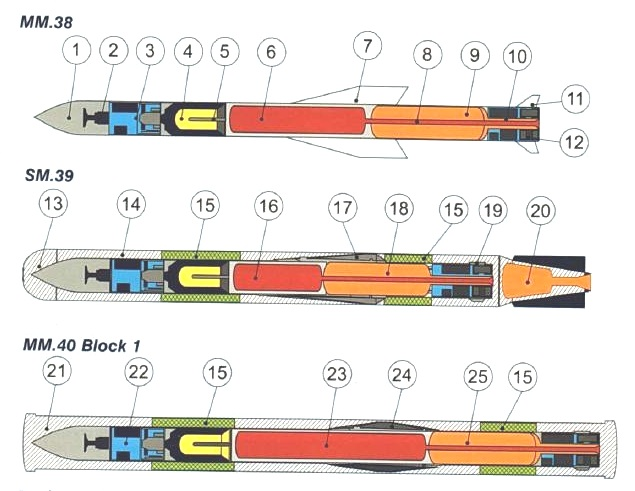
\includegraphics[width=0.9\textwidth]{images/exocetinterno.jpg}
\caption{Internal reference used to distribute mass by subsystem.}
\end{figure}

\begin{table}[H]
\centering
\caption{Mass distribution used in the 6DOF model.}
\begin{tabular}{lccc}
\toprule
Section & Length (m) & Structural mass (kg) & Propellant (kg) \\
\midrule
Control/seeker section & 0.70 & 70.0 & -- \\
Warhead & 0.95 & 165.0 & -- \\
Booster & 0.80 & 45.0 & 126.4 \\
Sustainer & 3.14 & 70.0 & 383.5 \\
Nozzle & 0.20 & 15.0 & -- \\
\bottomrule
\end{tabular}
\end{table}

With this distribution, the initial mass was 874.9 kg and the total length was 5.79 m. The calculated initial CG was 2.833 m, and the final CG after propellant burnout was 1.856 m.

The \(2.700~\text{m}\) value is therefore a common moment reference for the aerodynamic and 6DOF models, not the exact initial CG from the mass breakdown. The difference between the estimated initial CG and this reference is \(0.133~\text{m}\), or \(0.38\) calibers. Keeping one common moment reference avoids mixing aerodynamic and dynamic reference points, while the mass model itself still carries the time-varying CG used by the 6DOF simulation.

\begin{table}[H]
\centering
\caption{Initial and final inertia estimates used in the 6DOF model.}
\begin{tabular}{lcc}
\toprule
Parameter & Initial value & Final value \\
\midrule
Mass & 874.9 kg & 365.0 kg \\
\(X_{CG}\) & 2.833 m & 1.856 m \\
\(I_{xx}\) & 13.40 kg.m\(^2\) & 5.59 kg.m\(^2\) \\
\(I_{yy}=I_{zz}\) & 2155.40 kg.m\(^2\) & 863.30 kg.m\(^2\) \\
\bottomrule
\end{tabular}
\end{table}

The final CG value corresponds to complete propellant burnout. In the short 2.8 s 6DOF test, only the initial booster phase is represented; in that interval, the simulated CG moves from 2.833 m to 2.938 m because the early consumed propellant is located forward of the initial overall CG.
